
\section*{Mesh \& Hacking}
\DefineNamedColor{named}{eclipsered}{rgb}{0.186,0.166,0.182}
\definecolor{tablecolor}{named}{eclipsered}


\begin{eptable}{ l | X }
   \epheader{2}{General Usage}
   % Addiction & Needs fix or receive negative modifier.\\
   AR Mist & In ad-spammed area, up to \modifier{-30} general modifier.\\
   AR Filter & Counter AR mist with \skill{Interface} test.\\
   Hidden Tags & At least \skill{Interface} test at \modifier{-30} to find, maybe impossible.\\
   List Public Devices & Trivial activity.\\
   List Stealthed Devices & Opposed \skill{Interface} test at \modifier{-30} for searcher.\\
   Privacy Mode & Applies \modifier{-30} to tracking, might be illegal or frowned.\\
   Sniffing WiFi & Needs \textit{Sniffer} app, \skill{Hacking} test.\\
   Sniffing Laser & Needs to be in optical path.\\
   Sniffing Cabled & Needs hardware access.\\
   Sniffing VPNs & Applies \modifier{-30}, only valid for \dice{1d6} minutes.\\
   Sniffing Detection & Defender may make \skill{Infosec} test to detect every minute. \\
\end{eptable}

Selection of mesh actions that don't require a server account and have rules mentioned in the core book.
There are many other common mesh use cases (AR, VR, XP, Banking, Comms, Office, Networking, \ldots).

\bigskip

\subsection*{Accounts and Access}

These actions and rules are primarily concerned with systems (motes, hosts, servers) that have some sort of accounts,
and users that have gained or stolen access to these systems.

\begin{eptable}{ l | X }
   \epheader{2}{Accounts}
   % Addiction & Needs fix or receive negative modifier.\\
   Public Account & Does not require login, everyone has access.\\
   User Account & Requires authentication.\\
   Security Account & Can edit logs, modify other user data.\\
   Admin Account & Change all device features, services, shutdown.\\
\end{eptable}

\bigskip

\begin{eptable}{ l | X }
   \epheader{2}{Authentication Methods}
   % Addiction & Needs fix or receive negative modifier.\\
   Biometric Scan & Fingerprint, DNA, retina scan, \ldots\\
   Ego Scan & Brainwave scan with special device.\\
   Direct Neural Interface & Requires special brain implant.\\
   Mesh ID & Just needs the right mesh ID.\\
   Other Account & Account A might grant access to account B.\\
   Passcode & Some secret string, aka \textit{password}.\\
   Passkey & Special physical security token.\\
   Quantum Key & Require passcode delivered on highly secure channel.\\
\end{eptable}

\bigskip


\begin{eptable}{ l | X }
   \epheader{2}{Crypto}
   % Addiction & Needs fix or receive negative modifier.\\
   Public Key & Can be broken with quantum computer, \skill{Infosec} (1 week) task.\\
   Quantum & Cannot be broken, always requires key.\\
\end{eptable}

\bigskip

\begin{eptable}{ l | X }
   \epheader{2}{Universal Actions}
   Access System & Authenticate and access account.\\
   Apply Tag & Mark physical place or thing with AR tag.\\
   Communicate & Mail, text, chat if you have their mesh ID.\\
   Encrypt / Decrypt & Protect or access file if you have key.\\
   Filter AR Mist & Remove AR spam.\\
   Identify Attacker & Detect who is attacking you in mesh combat.\\
   Issue Command & Command a slaved device, ALI or bot with quick action.\\
   Log Off & Exit a system.\\
   Modify Files & Access, modify, delete files (might be recoverable).\\
   Operate Device & Control attached devices, might requires skill test.\\
   Run Script & Run pre-programmed script.\\
   Scan Wireless Signals & Try locate hidden or public devices and their mesh IDs.\\
   Search & Search connected system.\\
   Shield Software & Protect software targeted in mesh combat.\\
   Stealth WiFi Signals & Attempt to hide wireless activity.\\
   Switch Home Device & If infomorph, transfer mind to other system.\\
   Terminate Software & Kill software for which you have access.\\
   Toggle AR Skin & Change looks of world around you.\\
   Toggle Privacy Mode & Set your profile public or private.\\
   Toggle Simulspace & Enter or exit simulspace.\\
   Use Apps & Use installed app, may also require \skill{Interface} test.\\
   Use Service & Access cloud service for which you have access.\\
   View Apps & List all apps you have access to.\\
   View Profile & See profile and rep of anyone not in private mode.\\
   View Sensor Feeds & Access sensor, might also require \skill{Perception} or \skill{Know}.\\
   View System Status & View general system health and activity.\\
\end{eptable}

\bigskip


\begin{eptable}{ l | X }
   \epheader{2}{Security Actions}
   Acquire Mesh ID & View mesh ID of anyone accessing system.\\
   Activate Countermeasure & Trigger countermeasure against spotted attacker .\\
   Attack & Engage against other apps or users.\\
   Bypass Jamming & \skill{Interface} to get short (\SI{3}{s}) transmission through.\\
   Locate Intruder & Identify attacker to system.\\
   Lockout & Block ID (defeat in combat first if signed on).\\
   Monitor Activity & Watch user activity (might require \skill{Infosec}).\\
   Scan Infomorph & Reveal info about infomorph (\skill{Interface}).\\
   Trace & Trace user to physical location.\\
   Trigger Alert & Put system into passive or active alert.\\
   View Logs & View previous user activity.\\
   View Users & View all non-hidden users.\\
\end{eptable}

\bigskip

\begin{eptable}{ l | X }
   \epheader{2}{Admin Actions}
    Disable Systems & Turn off sensors or functions.\\
    Modify Accounts & Add, remove, modify accounts.\\
    Modify Privileges & Modify existing account permissions.\\
    Modify Software & Install, modify or remove software.\\
    Wipe System & Takes 1 to 10 minutes (double for secure wipe).\\
\end{eptable}



% \bigskip

% \begin{eptable}{ X }
%    \epheader{1}{What Your Muse Can}
%     Protect PAN as system defender, shield in mesh combat, launch countermeasures. \\
%     Make research tests to find information. \\
%     Falsify or fluctuate mesh ID. \\
%     Scan newsfeeds for keywords and alerts. \\
%     Teleoperate robots and ALIs. \\
%     xxx. \\
%     xxx. \\
%     xxx. \\
%     xxx. \\
%     xxx. \\
% \end{eptable}

\subsection*{Searches}

\begin{itemize}
   \itembox \textbf{Common Information}. Instant and does not require roll.
   \itembox \textbf{Uncommon Information}. On local mesh have timeframe of \SI{1}{h}, and might be complemented by appropriate \skill{Know} skill. Searches outside of the local mesh increase time frame due to distance lag.
   \itembox \textbf{Private Information}. (Located on specific host or sub-net) requires appropriate access and has special time frame (see table). Encrypted files must be decrypted before they can be searched.
   \itembox \textbf{Superior successes}. provide more nuanced information, \textbf{critical success} leads to breakthrough understanding, \textbf{critical failure} to false or misleading information.
   \itembox \skill{Research} only yields information. Understanding data might require \skill{Know} test or similar.
\end{itemize}


\begin{figure}[htbp!]%
   \centering
   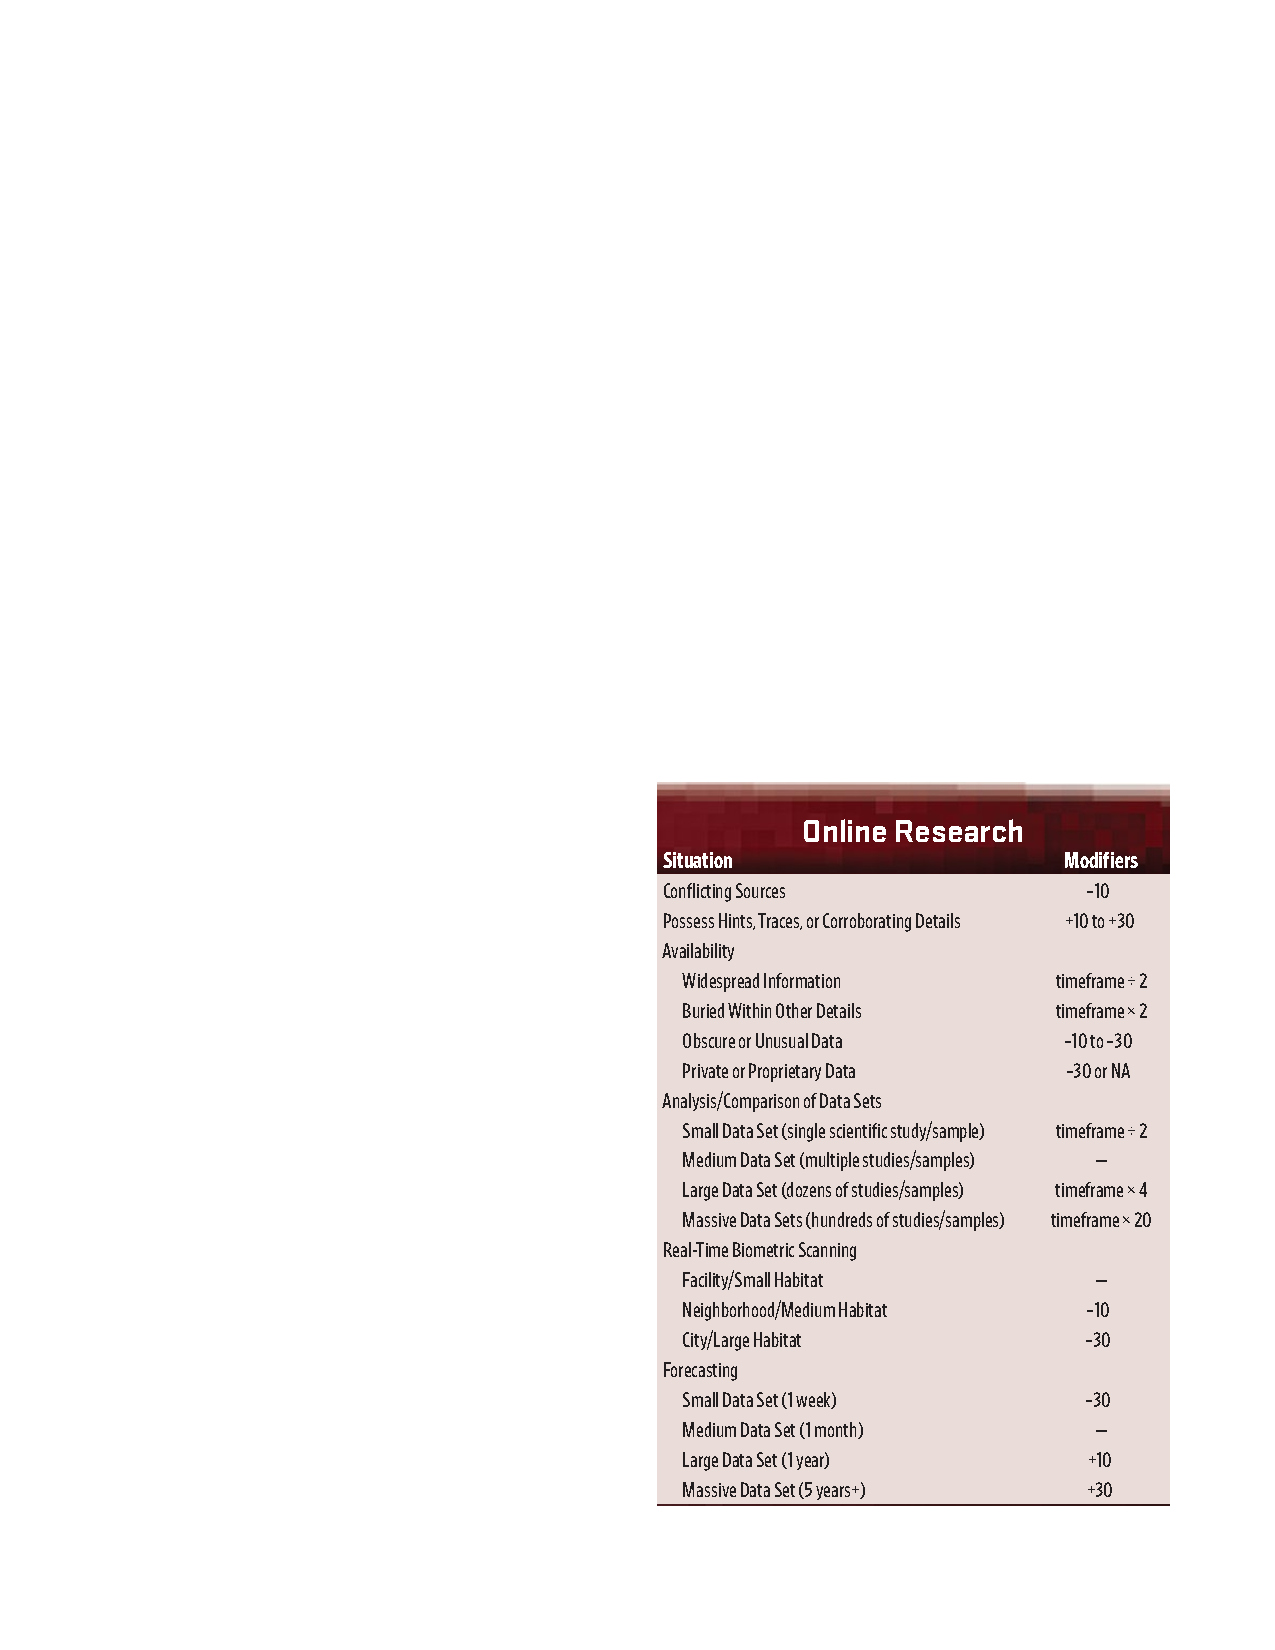
\includegraphics[scale=0.9]{gfx/mesh-research}%
\end{figure}%

\begin{figure}[htbp!]%
   \centering
   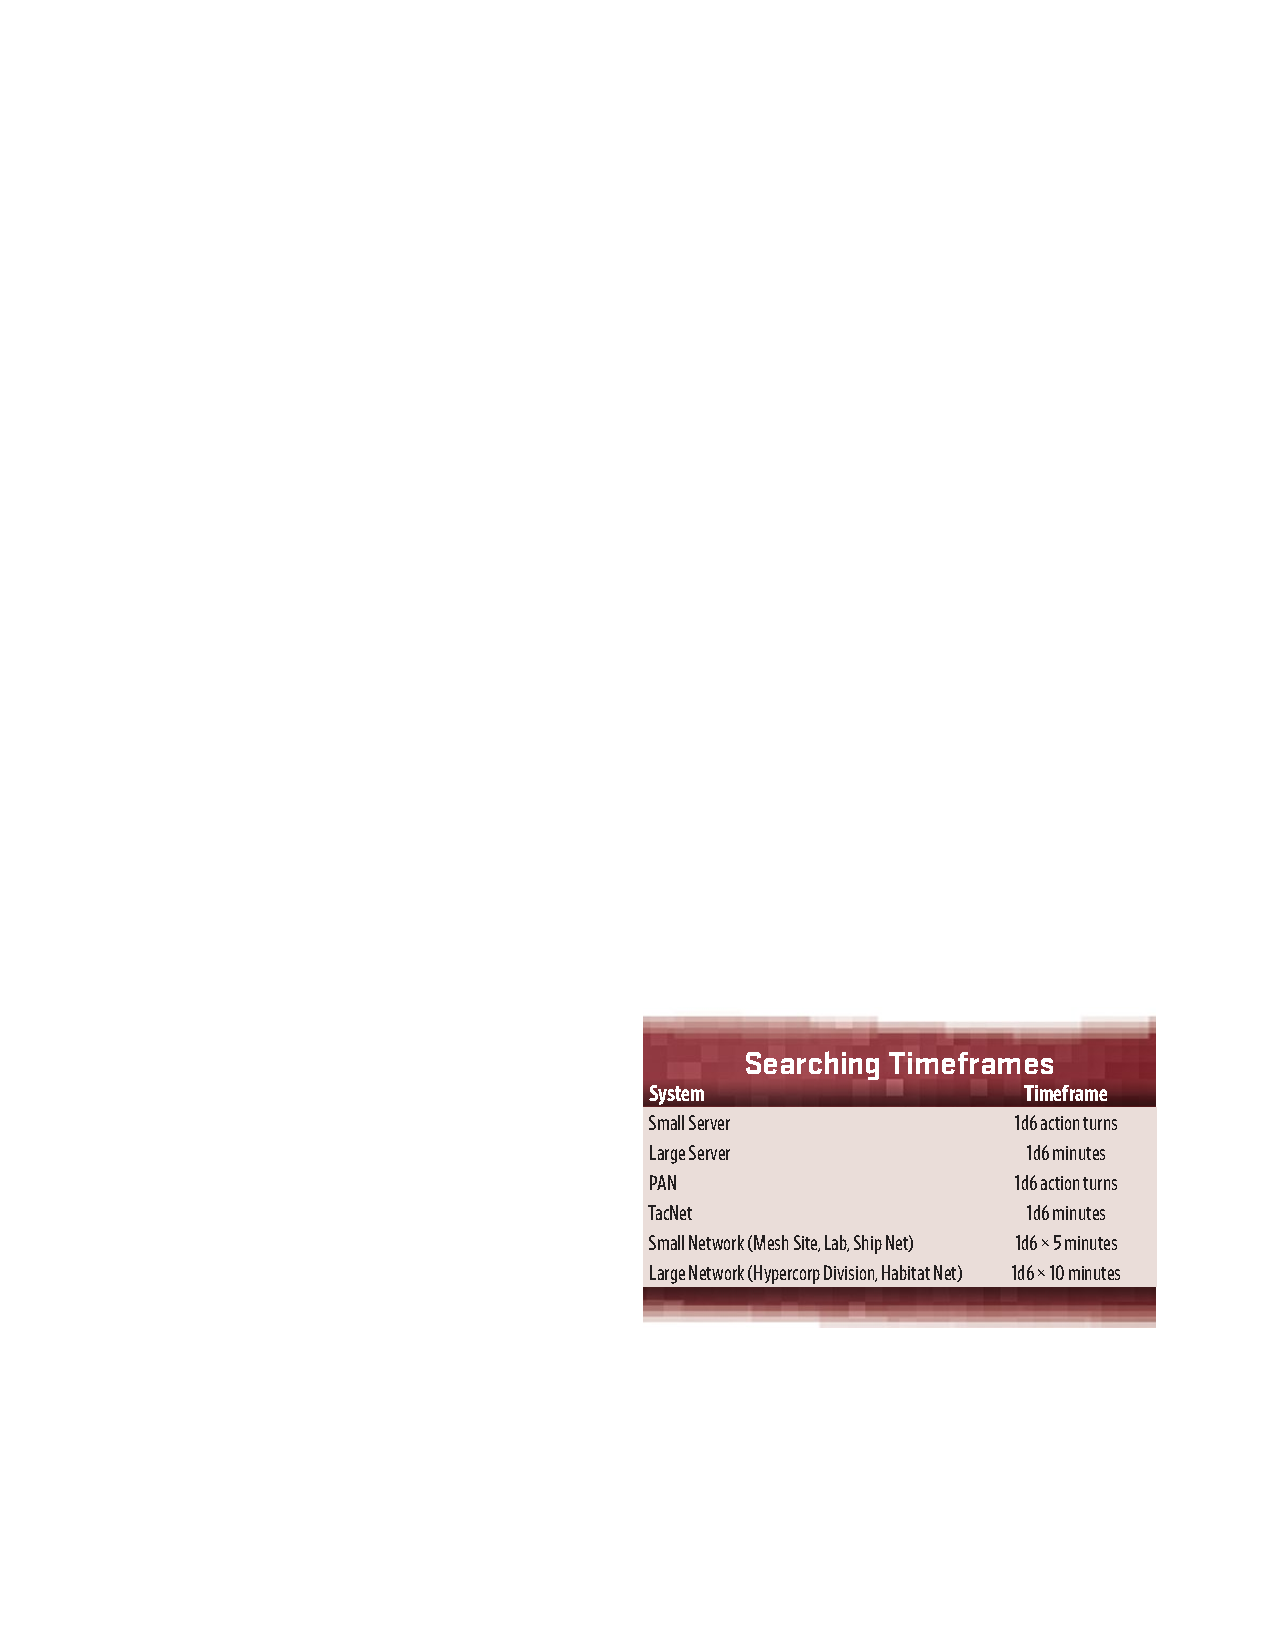
\includegraphics[scale=0.9]{gfx/mesh-search-time}%
\end{figure}%


\subsection*{Physical Tracking}

\begin{itemize}
   \itembox \textbf{Via Mesh ID}. \skill{Research} and can yield location of target and is instant. If they are in private mode \modifier{-30} modifer, opposed vs \skill{Infosec} if they cycle mesh IDs, timeframe \SI{1}{h}.
   \itembox \textbf{Via Biometrics}. Handled as \skill{Perceive} or \skill{Research}, possibly opposed by \skill{Infiltrate} or \skill{Disguise}.
\end{itemize}


\begin{figure}[htbp!]%
   \centering
   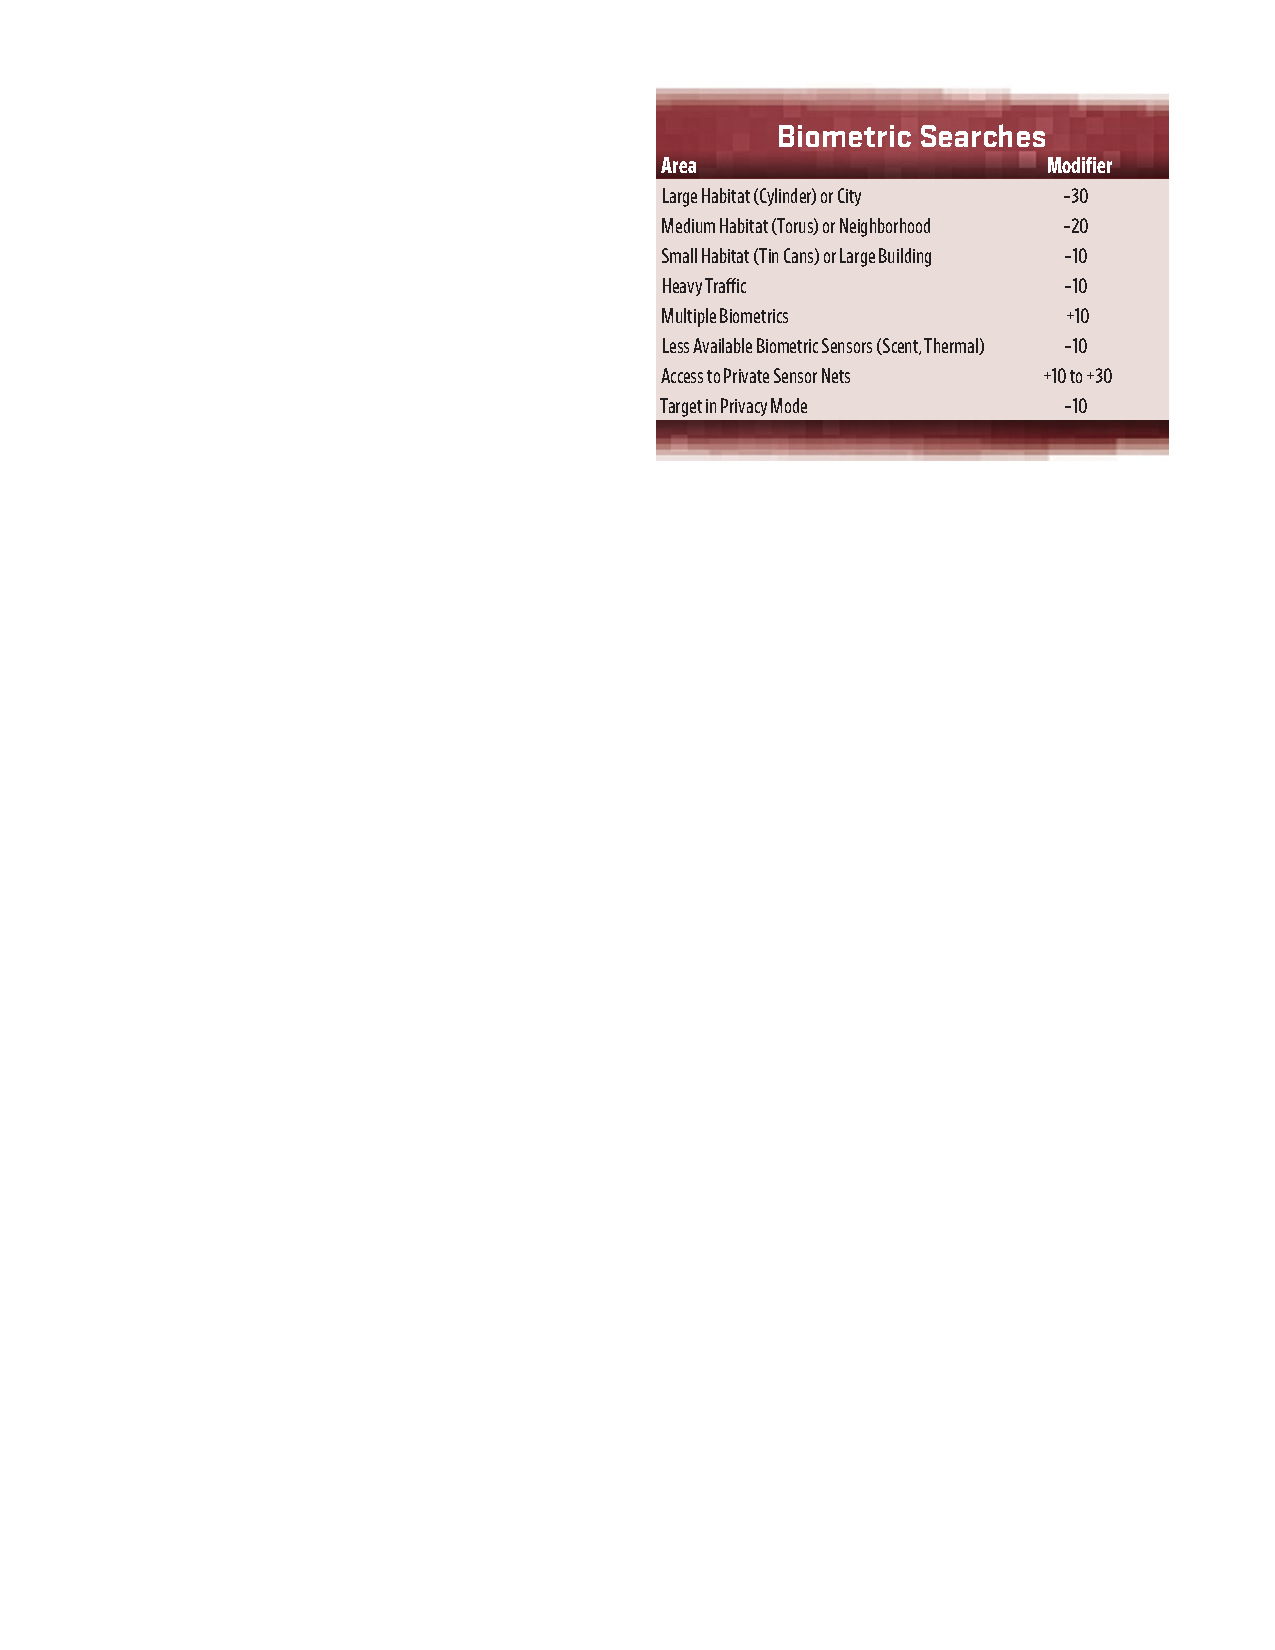
\includegraphics[scale=1.0]{gfx/mesh-search-biometric}%
\end{figure}%

\subsection*{Mesh Tracking}

\begin{itemize}
   \itembox \textbf{Live Activity Tracking}. Generally difficult (\skill{Research} at \modifier{-30}) or impossible even if mesh ID is known. Better approach is to sniff traffic or hack their PAN. Tracking activity on particular system can be done with elevated accounts.
   \itembox \textbf{Countermeasures}. Burner mesh IDs, disposable Ectos, VPNs, anonymizing proxies and spoofing mesh IDs.
   \itembox Public information easily accessible, private info might require \skill{Research} scraping at \modifier{-30}, favors, or special database access.
\end{itemize}


\subsection*{Breaking In}

\begin{eptable}{ l | X }
   \epheader{2}{Ways of Hacking}
   Acquiring Credentials & Get access to actual credential.\\
   Circumvent Authentication & Gain or forge access tokens.\\
   Spoofing & Intercept traffic and impersonate user.\\
   Intrusion & Find exploits to gain access.\\
\end{eptable}

\bigskip

% \begin{eptable}{ l | X }
%    \epheader{2}{Circumventing Authentication}
%    % Addiction & Needs fix or receive negative modifier.\\
%    Acquiring Credentials & Get access to actual credential.\\
%    Forging Authentication & Might require multiple tests and lengthy times.\\
%    Spoofing & Take over existing user connection, see below.\\
%    Intrusion & Exploit system weakness, see chapter below.\\
% \end{eptable}

\begin{itemize}
   \itembox Credentials usually do not raise alert. Spoofing or Intrusion might.
   \itembox \textbf{Hacking Basics}. Usually opposed roll between attacker \skill{Infosec} and system \skill{Firewall} (default protection) or defender \skill{Infosec} (if actively protected).
   \itembox \textbf{Spoofing}. Monitor active connection of existing user with sniffer. Then take over victim's client with \skill{Hacking} test, complex action. This \textit{only} allows sending. Victim VPN gives \modifier{-30}, Firewall can detect. To also take over victim's server for full-duplex, similar \skill{Hacking} test must succeed.
   \itembox \textbf{Intrusion Requirements}. Requires a direct connection to target, either wirelessly (need to know target mesh ID), via an access port, or via tapping into a cable (\skill{Hardware: Electronics}).
   \itembox \textbf{Intrusion (Brute Force)}. Complex action, opposed \skill{Hacking} at \modifier{-30}. If successful get user access level (1 superior gives security account, 2 give admin account). If successful attacker gets \textbf{spotted} status, system goes into \textbf{active alert}. On critical success \textbf{covert} status and \textbf{passive alert}. On failure no access and system goes \textbf{passive alert}.
   \itembox \textbf{Intrusion (Subtle)}. Takes \SI{1}{h} or longer task action. Success grants user access level (1 superior gives security account, 2 give admin account) and \textbf{covert status}. On critical success \textbf{hidden}. If firewall succeeds its roll (regardless whether it still loses opposed test) \textbf{passive alert} triggered.
   \itembox Remember to take time, use pools to redo rolls, or get extra mesh actions.
\end{itemize}

% \begin{figure}[htbp!]%
%    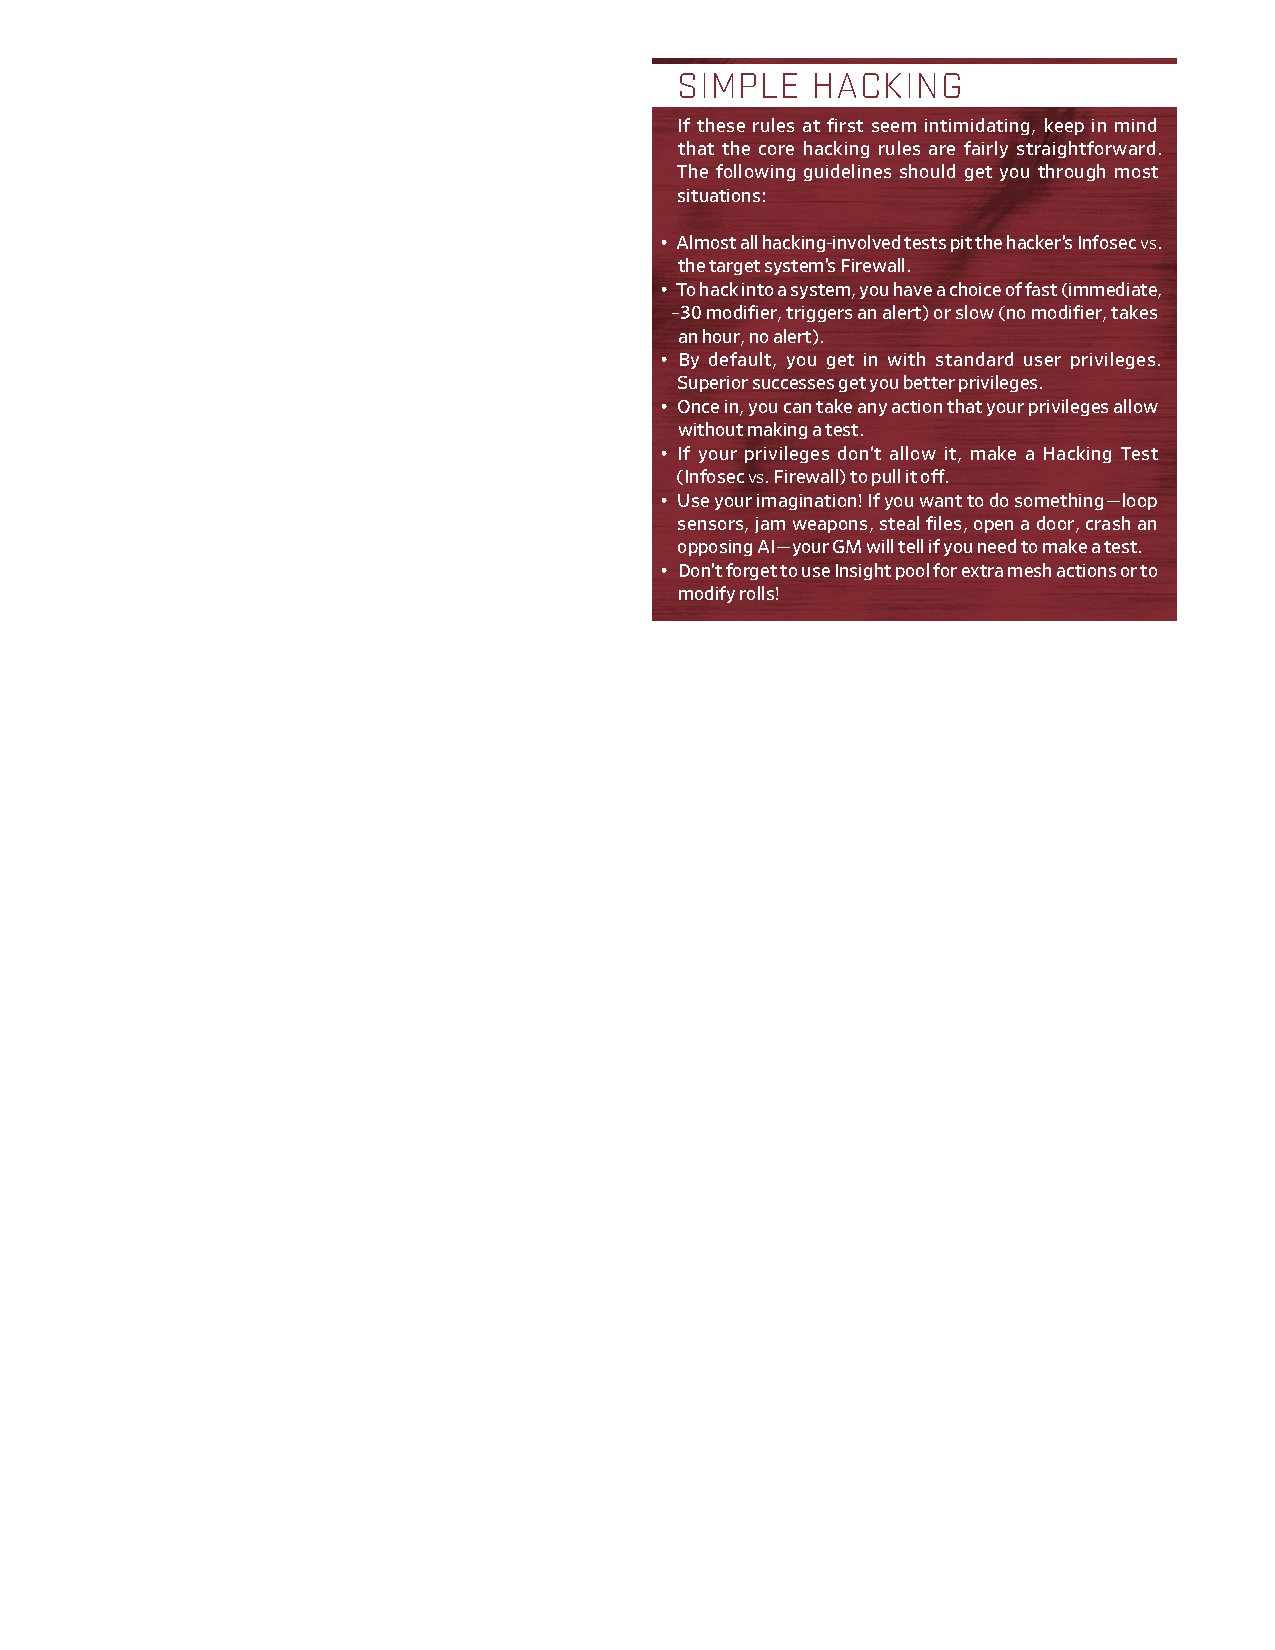
\includegraphics[scale=1.0]{gfx/mesh-hacking}%
% \end{figure}%


\begin{figure}[htbp!]%
   \centering
   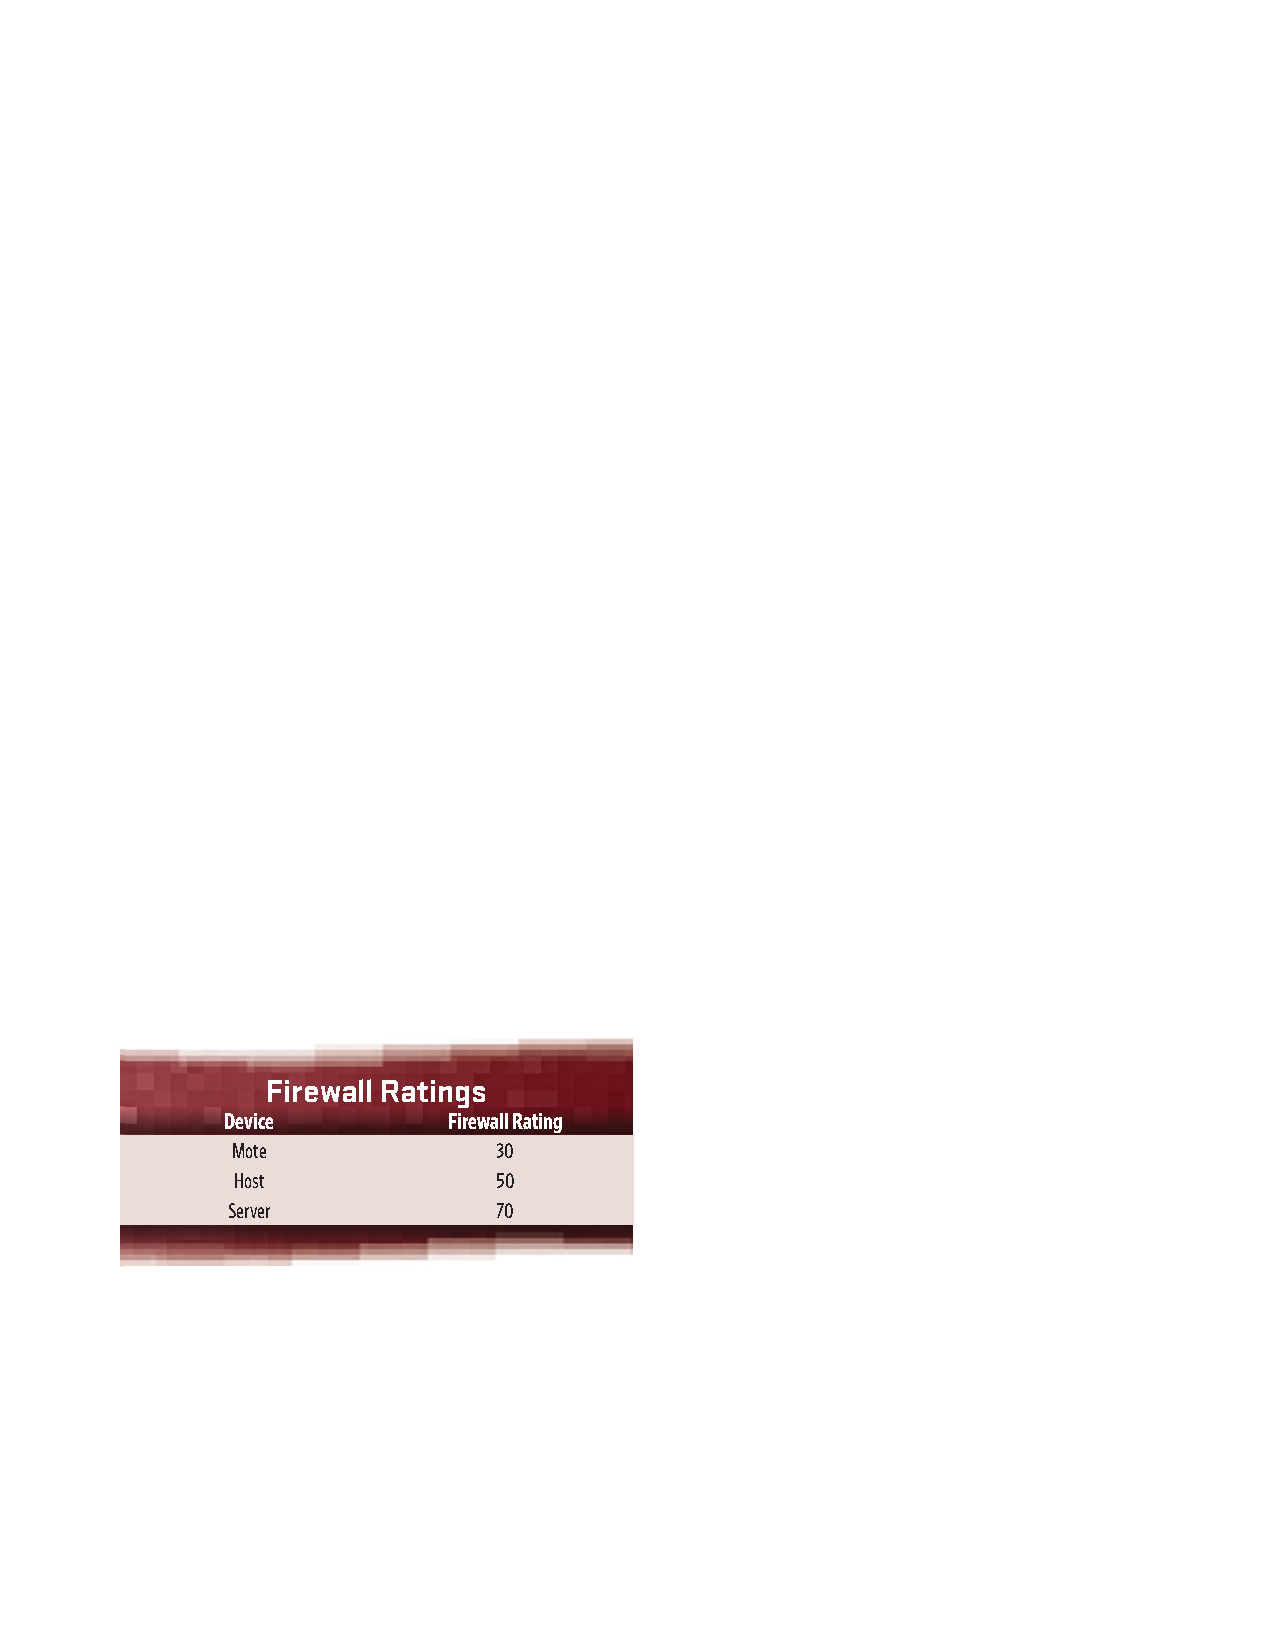
\includegraphics[scale=1.0]{gfx/mesh-firewall}%
\end{figure}%

\subsection*{Status \& Countermeasures}

\begin{eptable}{ l | X }
   \epheader{2}{Intruder Status}
    Hidden & System completely unaware, no logs, +10 to subvert system.\\
    Covert & System aware of presence, but does not consider threat.\\
    Spotted & System considers threat, active alert, launches countermeasures.\\
\end{eptable}

\bigskip

\begin{itemize}
   \itembox \textbf{Upgrade Status}. Can spend complex action \skill{Hacking}. Superior gives improves status by extra step. Does not erase logs or lower alert, but makes harder to pinpoint attacker.
   \itembox \textbf{Downgrade Status}. Any \skill{Infosec} while within system risks exposure, superior failure triggers \textbf{passive alert}, critical failure \textbf{spotted status}.
   \itembox \textbf{Zero In}. To take action against attacker, system needs to zero in. Pinpointing intruder on passive alert as opposed \skill{Infosec} against intruder. System suffers \modifier{-30} if intruder hidden. If successful, attacker \textbf{spotted}, system goes \textbf{active alert}.
\end{itemize}


\begin{eptable}{ l | X }
   \epheader{2}{Security Alerts}
    Passive Alert & Notifies admin, might launch passive CM, usually \SI{10}{m} cooldown.\\
    Active Alert & Launches active CM, attacker suffer \modifier{-10}.\\
\end{eptable}

\bigskip

\begin{eptable}{ l | X }
   \epheader{2}{Passive Countermeasures}
    Backup & Back up all critical information to prevent deletion.\\
    Egress Filtering & Block outgoing transfers (contest w. \skill{Hacking}).\\
    Locate Intruder & Try to zero in on intruder in system.\\
    Reduce Privileges & Reduce access rights of standard users.\\
\end{eptable}

\bigskip

\begin{eptable}{ l | X }
   \epheader{2}{Active Countermeasures}
    Counter Intrusion & Try to back-hack intruder if identified.\\
    Crash and Lockout & Crash intruder shell and prevent further access.\\
    Reboot or Shutdown & Takes \dice{1d6} actions or minutes.\\
    Terminate Connections & System can't be accessed anymore.\\
    Trace & Try to identify attacker's physical location.\\
\end{eptable}


\begin{figure}[htb!]%
   \centering
   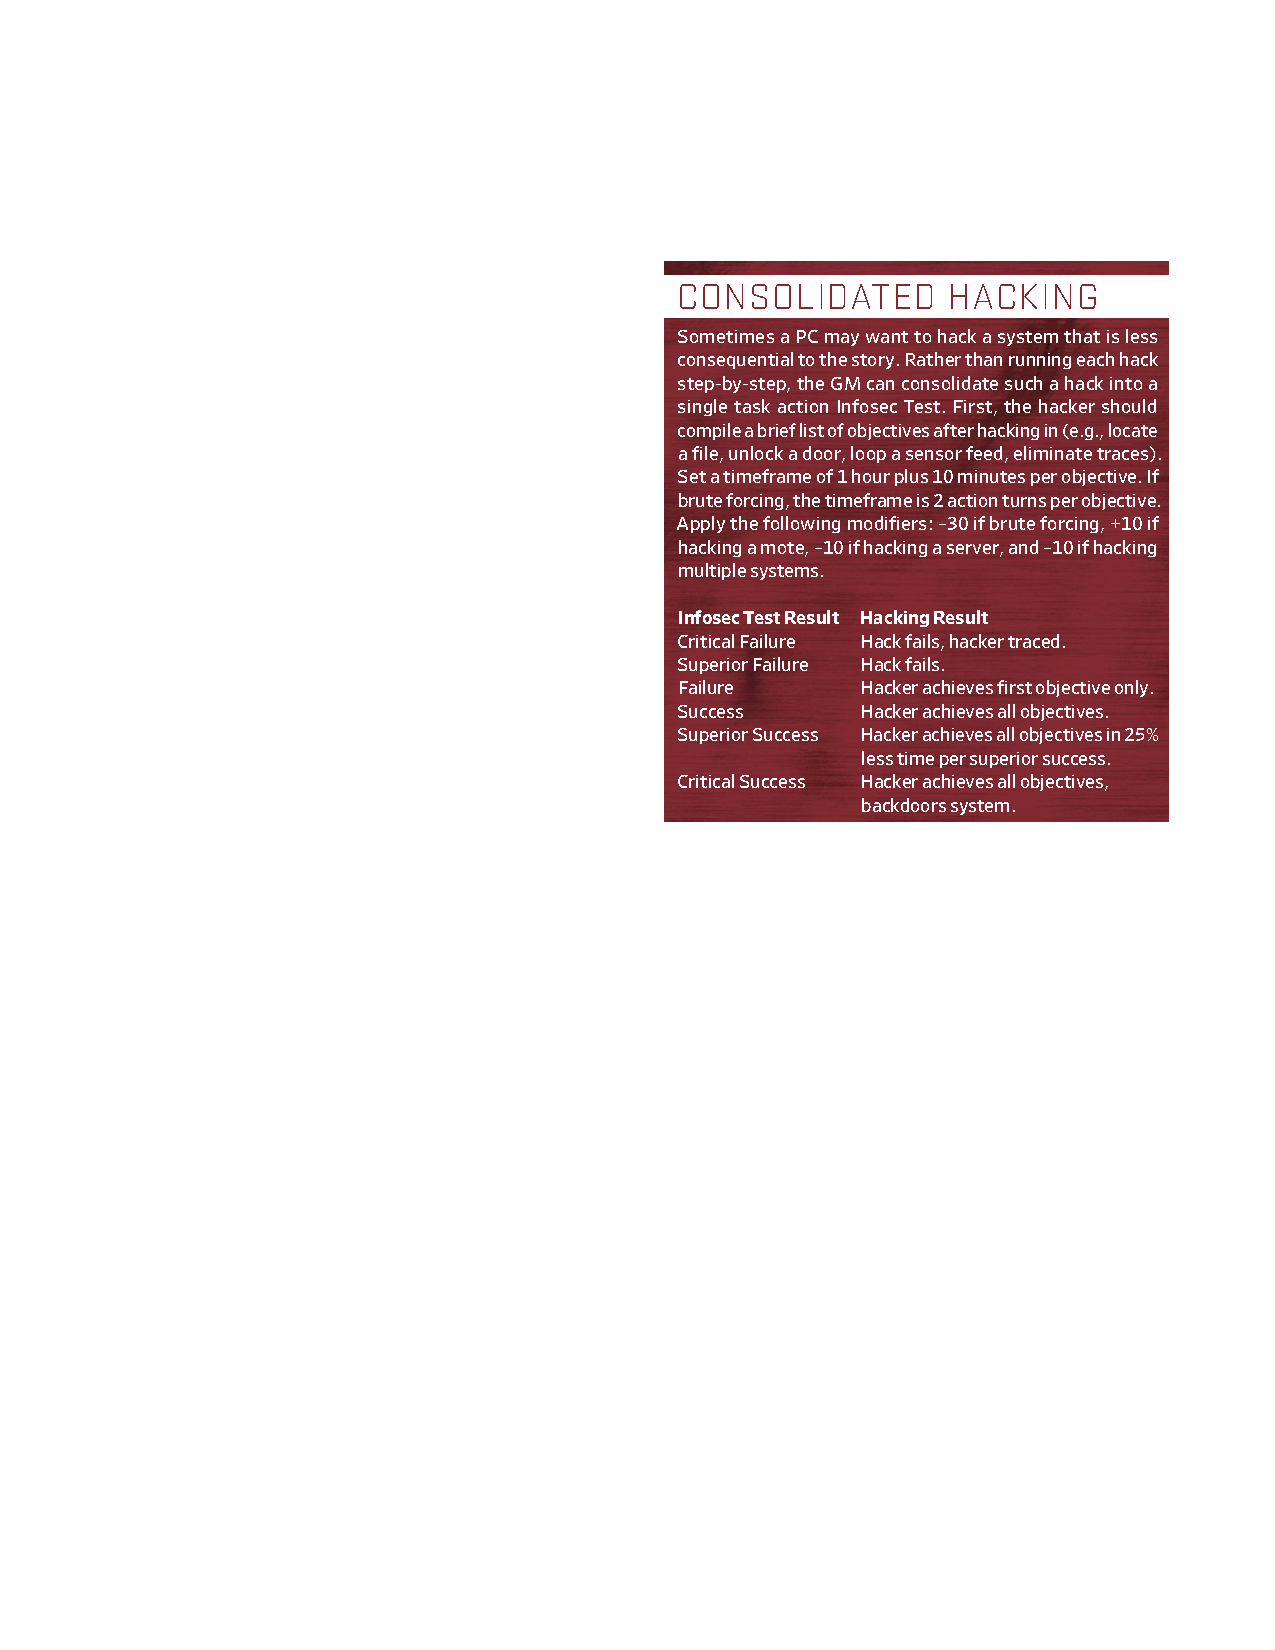
\includegraphics[scale=1.0]{gfx/mesh-consolidated-hacking}%
\end{figure}%

\bigskip

\subsection*{Subversion}

\begin{eptable}{ l | X }
   \epheader{2}{Subversion}
   Break Encryption & View all non-hidden users.\\
   Control Ware & Modify user hardware.\\
   Disable Safety Mechanics & Disable system preventing accidental harm.\\
   Edit AR Feed & Block or override user's sensory data.\\
   Eliminate Traces & Clean up evidence of break in.\\
   Force Re-Authentication & Can be used to sniff user's credentials.\\
   Hide File or Process & Makes it harder to find later.\\
   Impair Senses & Can induce \modifier{-10} modifiers to perception.\\
   Inject AR Illusion & Crafted in advance for best results.\\
   Install Backdoor & Bypass authentication later.\\
   Install Blocker & Block apps and countermeasures.\\
   Jam Signals & Interfere with local communications.\\
   Loop Sensor Feed & Undermine surveillance.\\
   Modify Tacnet & Change enemy's status information. \\
   Sniff Traffic & See above. \\
   Suppress Alarm & Turn off passive alarm or reduce active to passive. \\
   Suppress Process & Prevent process from coming back on again. \\
   Tap AR & See other user's AR feed as if it were your own. \\
   Tap Senses & Tap into cyberbrain or mesh insert senses. \\
\end{eptable}

Subversion are all activities that either try to bypass current permissions,
\textbf{or would generally be considered \textit{negative}} by defending firewall.
Usually handled as opposed \skill{Hacking} test.

\subsection*{Mesh Combat}

\begin{itemize}
   \itembox \textbf{Attacking (Local)}. Require access and account on system and can attack entities on system. In particular when \textbf{fighting active shell of spotted intruder} by system firewall or defender. Complex action \skill{Infosec} (\modifier{-30} if without admin account). If system shielded, opposed roll instead against \skill{Infosec}.
   \itembox \textbf{Attacking (Remote)}. Against operating systems of remote devices, but cannot attack infomorphs, cyberbrains, or software running on them. Opposed \skill{Infosec} against \skill{firewall} or defender's \skill{Infosec}.
   \itembox \textbf{Awareness}. Attacks not obvious to victim, look like glitches. Can't fight back unless aware, and \skill{Infosec} complex action to identify attacker. Attacks also require successful \skill{Hacking} test, or system goes into \textbf{passive alert}.
   \itembox \textbf{Damage}. Roll \dice{2d10}, add \dice{1d6} per superior, double for critical.
   \itembox \textbf{Wounds}. Like regular wounds if damage exceeds threshold. Induce cumulative \modifier{-10} modifier. Each wound causes cumulative \SI{10}{\%} chance for system glitch.
   \itembox \textbf{Healing}. Apps can't heal and need to restart. Infomorphs and others heal \dice{1d10} or 1 wound per minute.
\end{itemize}

\bigskip

\begin{eptable}{ l | X }
   \epheader{2}{Glitch Table}
    1 - 2 & Lost Connectivity. If cyberbrain, collapses or freezes.\\
    3 & Encoding Error. Might get spotted, leak real ID, compromise system.\\
    4 & Memory Loss. Might lose file, memory or skill until reboot.\\
    5 & Hung Process. App or synthmorph system might stop working.\\
    6 & Overload. Can't use pool for \dice{1d6}, or function every other round.\\
\end{eptable}


\begin{figure}[htb!]%
   \centering
   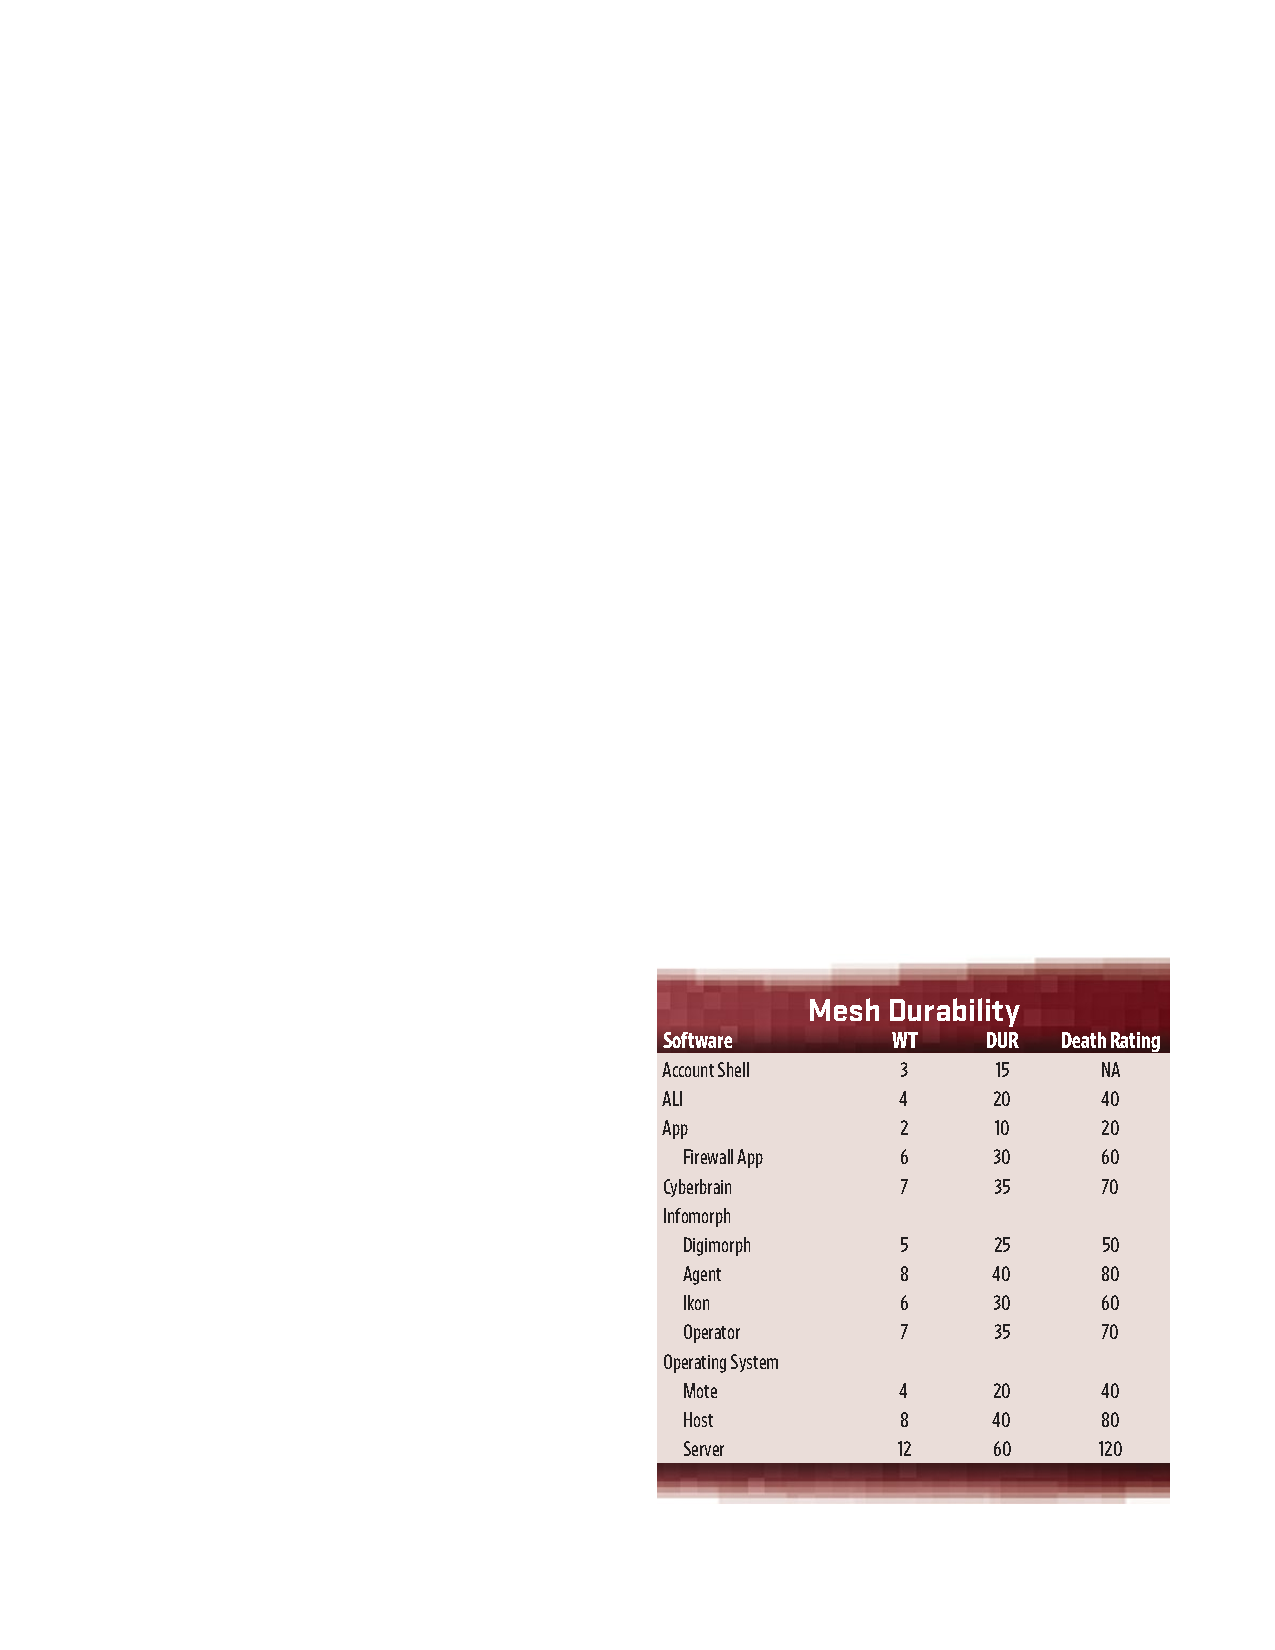
\includegraphics[scale=1.0]{gfx/mesh-combat}%
\end{figure}%


\subsection*{Counter-Surveillance}

\begin{itemize}
   \itembox \textbf{Detecting Sensors}. Many sensors radiate WiFi publically, private ones can be triangulated with \skill{Interface} (\modifier{-30}). \skill{Perception} (up to \modifier{-30}) to see sensors, depending on if active or passive.
   \itembox \textbf{Hacking Sensors}. Single sensor like regular hacking. Mass hacking can work, as motes have bad security. Treat as \textbf{consolidated hacking} with \modifier{-10} per \num{5} sensors.
   \itembox \textbf{Avoiding Recognition}. Use devices like shrouds, invisibility cloaks, masks, chameleon skin, disguises, and many more. Might yield opposed \skill{Infiltrate} or \skill{Disguise} against system's \skill{Perceive} (applying negative modifiers).
   \itembox \textbf{Disabling Sensors}. Jam to prevent certain sensors from transmitting, not necessarily recording though. Permanently disables sensors via EMP or similar until replaced. Alternatively, carefully removing sensors if task \skill{Perception} roll if you don't mind to be seen, or \skill{Infiltrate} with double time frame to do covertly. Spy nanoswarms require separate cleaning with guardian swarms.
   \itembox \textbf{Dead Zones \& Route Mapping}. Many places have no sensor coverage due to age, environment, vandalism. Route mapping (finding a dead zone path) treated as task \skill{Infiltrate} with modifiers based on area. Black market might sell \textit{dead zone maps}.
   \itembox \textbf{Skipjacking}. Moving while under surveillance without raising suspicion is \skill{Infiltrate} with modifiers based on area, opposed by \skill{Perceive}.
\end{itemize}